\subsection{3. 仿真与实验}\label{sec:experiments}

\subsubsection{3.1 实验配置与评价口径}\label{sec:experimental-scope}

实验固定采用一套代表性 DUV 配置，以避免不同参数组合干扰平台对比。目标 FPGA 为 Xilinx Kintex UltraScale+ xcku5p-ffvb676-2-e，设计使用 Vitis HLS 2025.2 和 Vivado 2025.2 实现，工作频率统一按 250 MHz 计算。软件性能基准运行于 Intel Xeon Platinum 8163 服务器，C++ 程序采用 C++17、单精度浮点和 \texttt{-O2} 优化，并链接 FFTW 3.x、LAPACK、BLAS 和 OpenMP 运行库。实验配置见表 4。

\textbf{表 4} 固定实验配置与比较口径

\begin{table}[htbp]
\centering
\small
\begin{tabular}{p{0.16\linewidth}p{0.76\linewidth}}
\toprule
类别 & 固定配置 \\
\midrule
光学与输入 & $L_x=L_y=1024$，$NA=0.8$，$\lambda=193$ nm，Annular 光源，$\sigma_{in}=0.6$，$\sigma_{out}=0.9$ \\
SOCS 配置 & 10 个 $17\times17$ 本征核，固定 $128\times128$ FFT 网格 \\
FPGA & xcku5p-ffvb676-2-e，Vitis HLS/Vivado 2025.2，250 MHz \\
CPU 基准 & Intel Xeon Platinum 8163 @ 2.50 GHz，GCC 13.3.0，C++17，单精度，\texttt{-O2} \\
精度基准 & MATLAB 完整 TCC 与 10 核 SOCS 高精度结果 \\
性能基准 & C++ 10 核 SOCS 在线重构，与 FPGA 执行相同输入和相同成像方程 \\
\bottomrule
\end{tabular}
\end{table}

本文将精度与性能采用不同但相互独立的参考口径。MATLAB 用于判断 10 核 SOCS 相对完整 TCC 的模型误差；同配置 SOCS software Golden 用于隔离 FPGA 定点量化、块浮点缩放和数据格式转换产生的硬件实现误差。加速比仅比较 C++ 与 FPGA 的相同 10 核在线 SOCS 算子，不包含离线 TCC 构建、特征分解、PCIe 传输和主机侧傅里叶插值。

\subsubsection{3.2 与 MATLAB 的精度验证}\label{sec:matlab-accuracy}

给定待验证图像 $X$ 和参考图像 $Y$，本文使用均方根误差衡量整体偏差：

\[
\mathrm{RMSE}(X,Y)=\sqrt{\frac{1}{N}\sum_{i=1}^{N}(X_i-Y_i)^2}.
\qquad\text{(11)}
\]

表 5 将模型截断误差与硬件实现误差分开报告。MATLAB 10 核 SOCS 与完整 TCC 直接成像之间的 RMSE 为 $5.472\times10^{-3}$，PSNR 为 36.95 dB，二值图形一致率为 98.77\%。该结果给出了固定 10 核模型相对高精度物理参考的误差边界。FPGA 板上 $128\times128$ 输出与同配置 SOCS software Golden 的 RMSE 为 $2.93\times10^{-8}$；结果经主机傅里叶插值恢复为 $1024\times1024$ 后，RMSE 为 $2.95\times10^{-8}$，PSNR 为 142.20 dB。

\textbf{表 5} 固定 10 核配置下的精度验证结果

\begin{table}[htbp]
\centering
\scriptsize
\begin{tabular}{p{0.19\linewidth}p{0.22\linewidth}p{0.13\linewidth}p{0.12\linewidth}p{0.10\linewidth}}
\toprule
验证对象 & 参考对象 & RMSE & MaxAE & PSNR \\
\midrule
MATLAB 10 核 SOCS & MATLAB 完整 TCC & $5.472\times10^{-3}$ & $9.821\times10^{-3}$ & 36.95 dB \\
FPGA 板上 $128\times128$ 输出 & 同配置 SOCS software Golden & $2.93\times10^{-8}$ & $3.58\times10^{-7}$ & 142.26 dB \\
FPGA+Host FI $1024\times1024$ 输出 & 同配置 SOCS software Golden & $2.95\times10^{-8}$ & $4.17\times10^{-7}$ & 142.20 dB \\
\bottomrule
\end{tabular}
\end{table}

FPGA 输出的实现误差比 10 核 SOCS 的模型截断误差低约五个数量级，说明最终空中像相对 MATLAB 完整 TCC 的偏差主要由低秩截断决定，而不是由 FPGA 数据通路引入。C/RTL 联合仿真的 RMSE 为 $8.324\times10^{-7}$，同样低于 $10^{-5}$ 的实现误差阈值。图 3 给出固定配置下的参考图像、FPGA 输出及误差分布，二者的主要成像结构保持一致。

\begin{figure}[htbp]
\centering
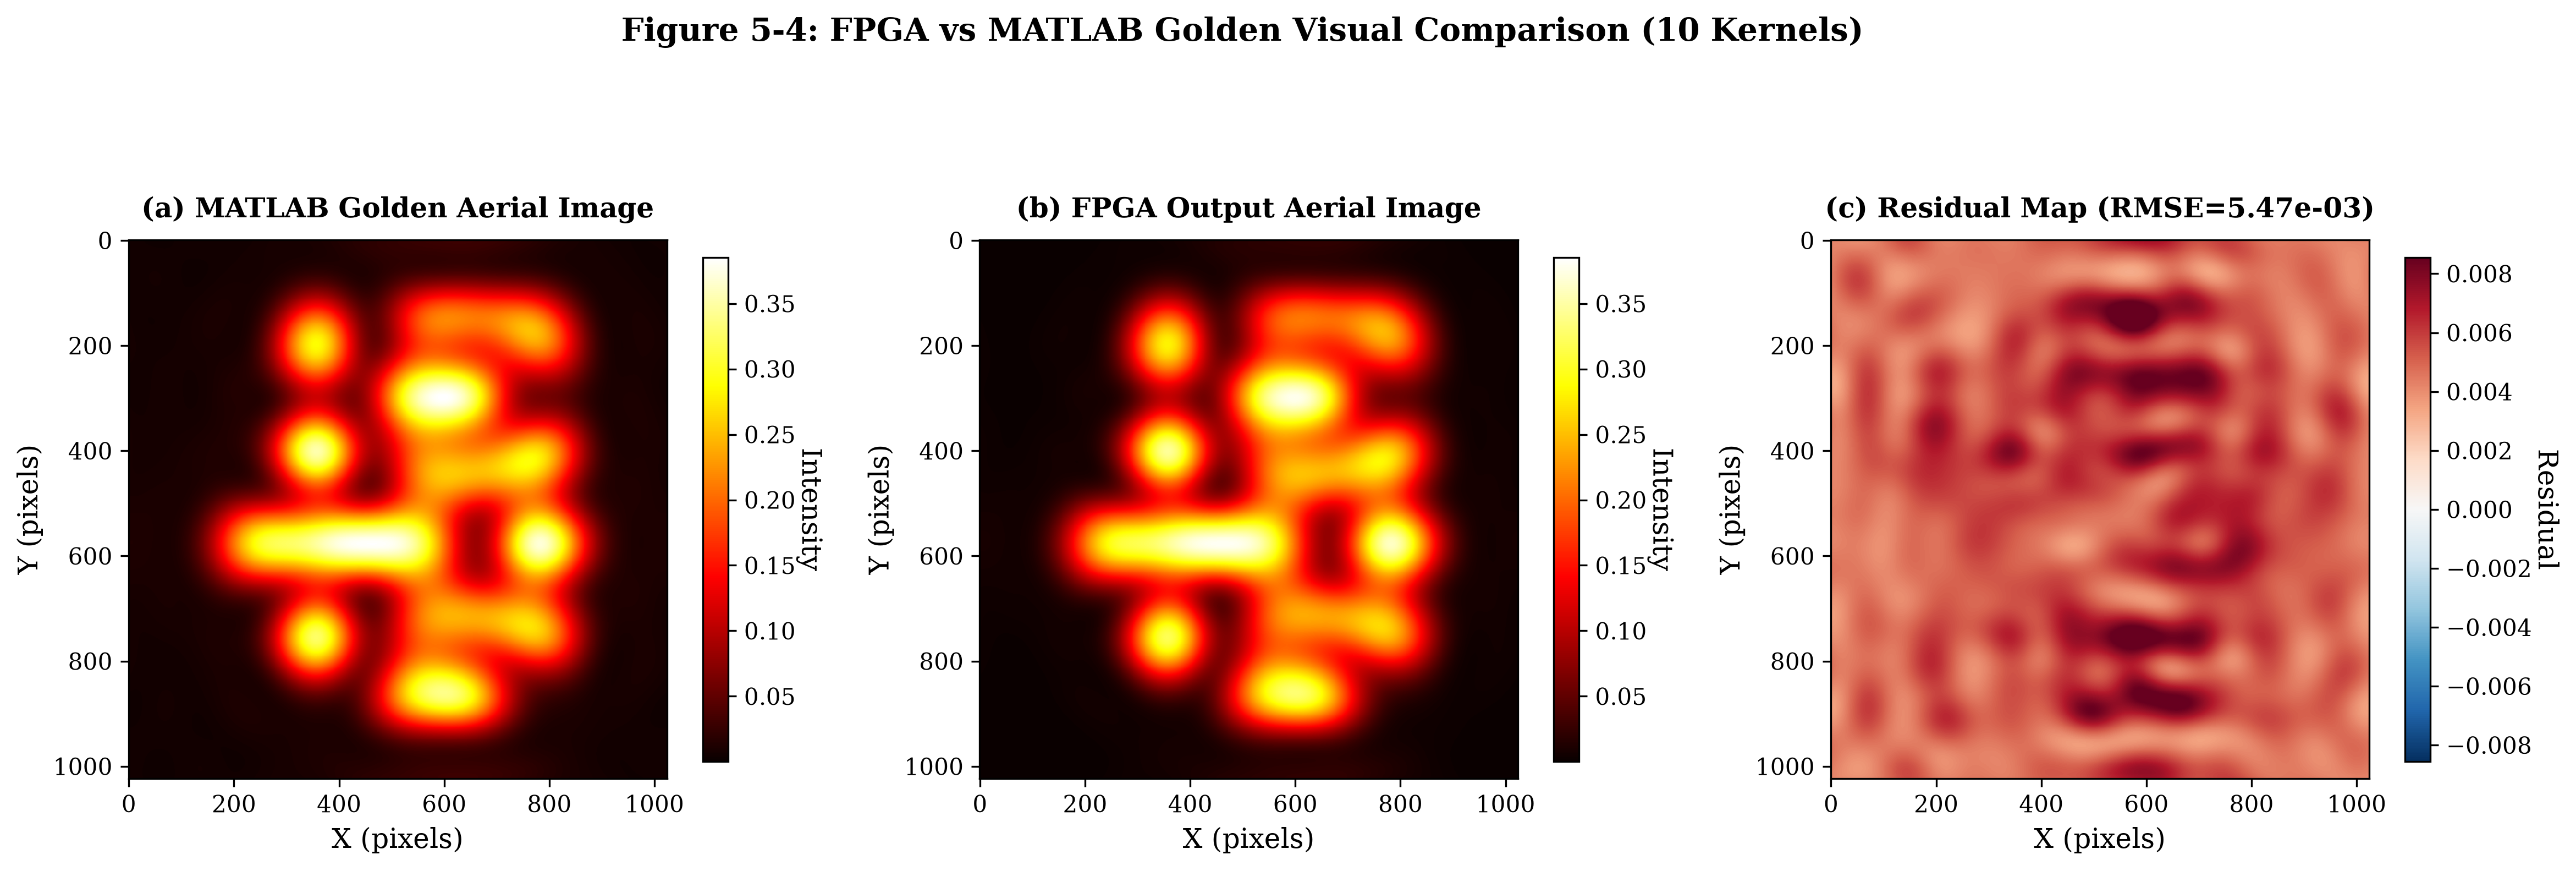
\includegraphics[width=\linewidth]{../image/论文/ch5_fig4_visual_comparison.png}
\caption{固定 10 核配置下的参考空中像、FPGA 输出与误差分布。}
\end{figure}

\subsubsection{3.3 加速比与能效比分析}\label{sec:speed-energy}

\paragraph{3.3.1 FPGA 内核延迟}

在 250 MHz 下，HLS 综合报告的顶层延迟为 2,643,645 个周期，对应 10.57 ms；C/RTL 联合仿真报告为 2,651,856 个周期，对应 10.61 ms。两者相差约 0.3\%，说明综合估计能够代表生成 RTL 的执行周期。表 6 给出 FPGA 内核的阶段分解。

\textbf{表 6} 10 核 SOCS 在线重构内核延迟分解。该表为 250 MHz 下的 kernel-only latency，不包含 PCIe 传输和主机 FI。

\begin{table}[htbp]
\centering
\begin{tabular}{lrrr}
\toprule
阶段 & 周期数 & 250 MHz 下时间 & 占比 \\
\midrule
频域嵌入，10 核 & 167,450 & 0.67 ms & 6.3\% \\
二维 IFFT，10 核 & 2,262,250 & 9.05 ms & 85.6\% \\
累加，10 核 & 164,250 & 0.66 ms & 6.2\% \\
FFTshift & 16,389 & 0.066 ms & 0.6\% \\
DDR 输出 & 16,389 & 0.066 ms & 0.6\% \\
\textbf{总计} & \textbf{2,643,645} & \textbf{10.57 ms} & \textbf{100\%} \\
\bottomrule
\end{tabular}
\end{table}

二维 IFFT 占总延迟的 85.6\%，是当前在线重构的主要性能瓶颈；频域嵌入和强度累加分别仅占 6.3\% 和 6.2\%。因此，固定网格复用、片上转置和 IFFT 数据通路优化直接决定整体延迟。

\begin{figure}[htbp]
\centering
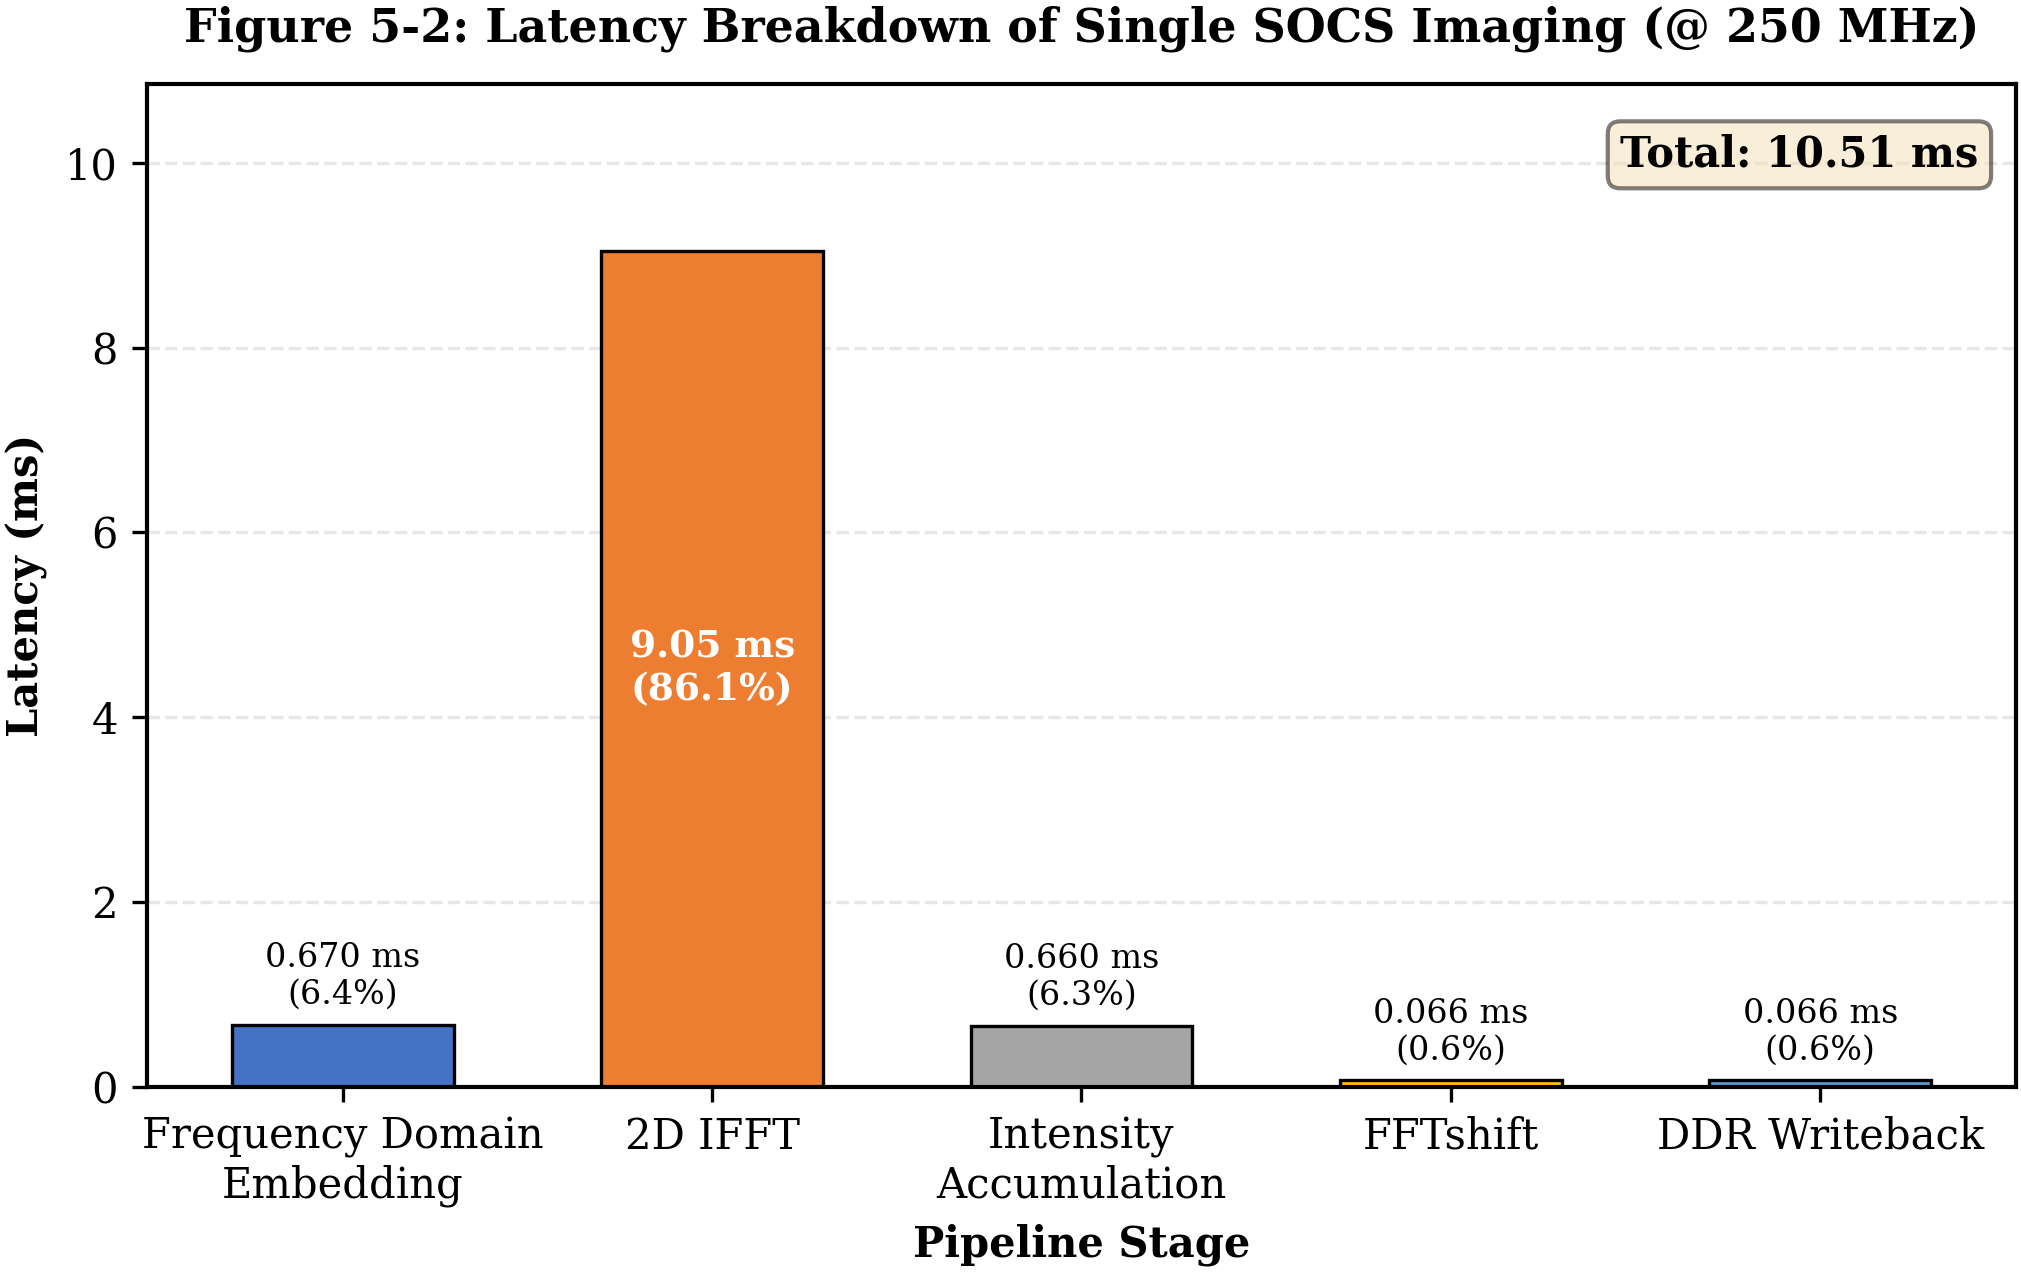
\includegraphics[width=\linewidth]{../image/论文/ch5_fig2_latency_breakdown.png}
\caption{所提出 FPGA 在线重构内核的延迟分解。}
\end{figure}

\paragraph{3.3.2 CPU-FPGA 加速比}

表 7 仅比较相同输入和相同 10 核 SOCS 方程下的在线重构阶段。C++ CPU 实测延迟为 35.6 ms，FPGA 内核延迟为 10.57 ms，因而实现 3.37 倍加速，单次延迟降低 70.3\%。对应吞吐量由 28.09 images/s 提升至 94.6 images/s。该比较不使用 MATLAB 运行时间或完整 TCC 直接成像时间，避免算法范围和实现精度不同造成不公平结论。

\textbf{表 7} 相同 10 核 SOCS 在线重构算子的 CPU-FPGA 性能对比

\begin{table}[htbp]
\centering
\begin{tabular}{lrrrr}
\toprule
平台 & 延迟 & 吞吐量 & 相对加速比 & 延迟降低率 \\
\midrule
C++ CPU SOCS & 35.6 ms & 28.09 images/s & $1.00\times$ & - \\
FPGA SOCS 内核 & 10.57 ms & 94.6 images/s & $3.37\times$ & 70.3\% \\
\bottomrule
\end{tabular}
\end{table}

这一加速收益来自执行结构而不是成像模型变化。CPU 通过软件循环依次执行复数乘法、二维 IFFT 和强度累加；FPGA 则复用固定尺寸 IFFT 引擎，并通过流水化循环、BRAM 中间缓冲和独立 AXI-MM 通道降低控制与访存开销。对于 OPC/SMO/ILT 中反复调用的窗口级空中像计算，单次 24.99 ms 的延迟节省可随调用次数累积。

\paragraph{3.3.3 单幅能耗与能效}

为比较单位任务的能耗，本文按 $E=P\times T$ 计算每幅空中像的能量消耗。当前 CPU 功耗采用约 80 W 的服务器运行功耗估计，FPGA 采用约 4 W 的 online reconstruction kernel 后综合功耗估计。因此：

\[
E_{\mathrm{CPU}}=80\times35.6\ \mathrm{ms}=2.848\ \mathrm{J/image},
\qquad\text{(12)}
\]

\[
E_{\mathrm{FPGA}}=4\times10.57\ \mathrm{ms}=0.0423\ \mathrm{J/image}.
\qquad\text{(13)}
\]

表 8 表明，在这一估算口径下，FPGA 单幅能耗降低约 98.5\%，能效由 0.351 images/J 提升至 23.7 images/J，对应约 67.4 倍的 kernel-level 能效提升。

\textbf{表 8} FPGA 与 C++ CPU SOCS 的估算内核能效对比

\begin{table}[htbp]
\centering
\begin{tabular}{lrrrr}
\toprule
平台 & 延迟 & 估算功耗 & 单幅能耗 & 能效 \\
\midrule
C++ CPU SOCS & 35.6 ms & 约 80 W & 2.848 J/image & 0.351 images/J \\
FPGA SOCS 内核 & 10.57 ms & 约 4 W & 0.0423 J/image & 23.7 images/J \\
\bottomrule
\end{tabular}
\end{table}

上述 67.4 倍仅表示基于当前功耗估计的 FPGA kernel-level energy efficiency，不代表 Host CPU、PCIe、DDR 和主机侧 FI 在内的全平台实测能效。投稿前仍需使用带活动信息的 Vivado Power Analyzer 报告或板上传感器校准 FPGA 功耗，并使用 RAPL、BMC 或外部功率计测量 CPU 基准功耗。

\paragraph{3.3.4 资源与系统边界}

最终设计的资源利用率见表 9。DSP 使用率仅为 2\%，说明 LUT 映射 FFT 乘法有效避免了 DSP 成为实现瓶颈；BRAM 使用率为 42\%，主要用于二维 IFFT 转置与多核累加缓冲。该资源分布使设计能够部署在中等规模 xcku5p 器件上，并为低功耗运行提供硬件基础。

\textbf{表 9} xcku5p 上的 FPGA 资源利用率

\begin{table}[htbp]
\centering
\begin{tabular}{lrrr}
\toprule
资源 & 使用量 & 可用量 & 利用率 \\
\midrule
LUT & 36,931 & 216,960 & 17\% \\
FF & 38,703 & 433,920 & 9\% \\
DSP & 34 & 1,824 & 2\% \\
BRAM\_18K & 399 & 960 & 42\% \\
\bottomrule
\end{tabular}
\end{table}

\begin{figure}[htbp]
\centering
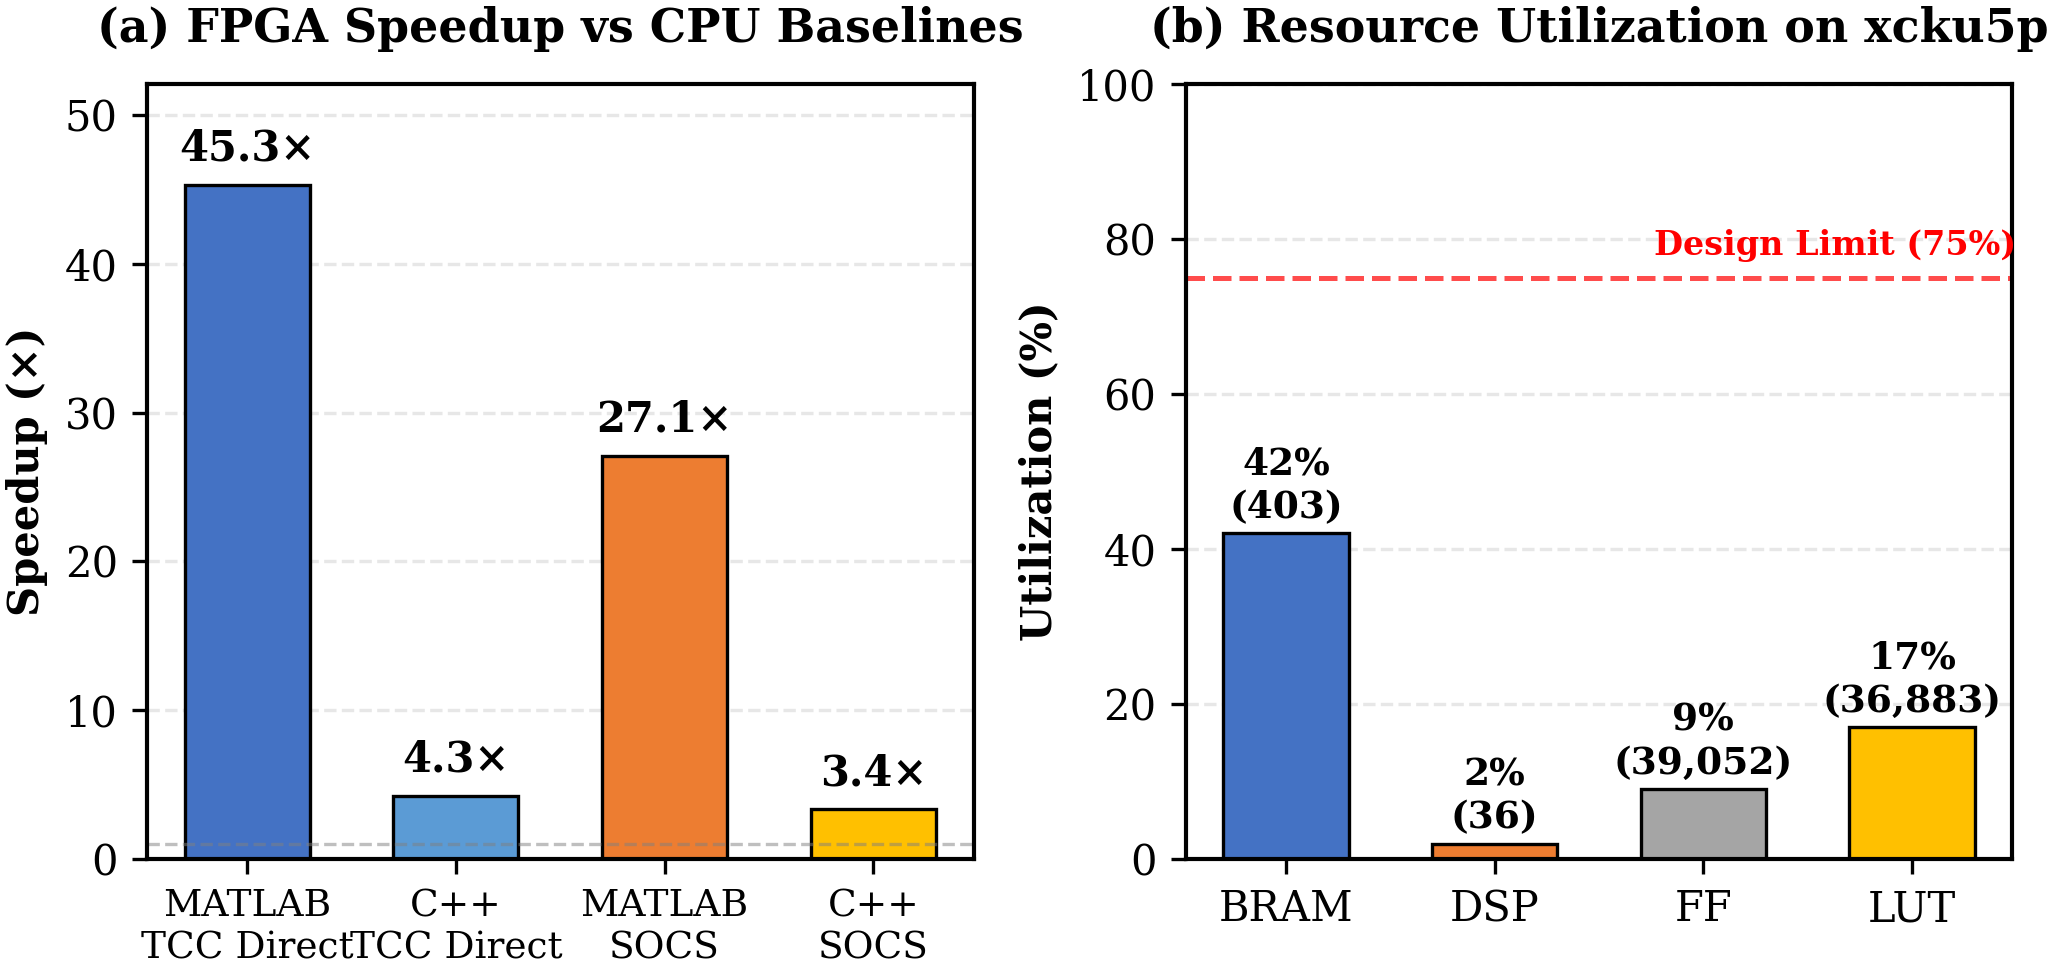
\includegraphics[width=\linewidth]{../image/论文/ch5_fig3_performance_resource.png}
\caption{所提出 FPGA/HLS 架构的性能、估算内核能效与资源总结。}
\end{figure}

本文还完成了 PCIe XDMA 板上数据写入、AXI-Lite 控制、结果回读和 Host FI 验证。该单窗口系统路径包含主机系统调用、DMA、轮询和后处理，其计时口径不同于表 7 的纯计算阶段，因此不参与 3.37 倍内核加速和 67.4 倍估算内核能效的计算。GPU 更适合追求大批量绝对吞吐的计算光刻任务；本文不以非同源公开数据进行定量优劣比较，而将所提出架构定位为低功耗、确定性延迟的在线重构内核。

综上，固定配置下的实验形成了完整证据链：MATLAB 对比给出 10 核 SOCS 的模型精度边界，板上验证表明 FPGA 实现误差远小于该边界，同算子 CPU 对比则证明 FPGA 能够在保持成像结果的同时降低在线延迟和估算单幅能耗。该结论仅适用于 TCC-SOCS online reconstruction kernel，不外推为完整 OPC/SMO 工具链或 Host-FPGA 全系统的能效结论。
